% -*- latex -*- This is a LaTeX document.
% $Id: scool05.tex,v 1.16 2005-10-06 14:41:12 cananian Exp $
%%%%%%%%%%%%%%%%%%%%%%%%%%%%%%%%%%%%%%%%
\documentclass{csa-sig-alternate}
\usepackage{epsfig}
%\usepackage{supertech}
\usepackage{array}
\usepackage{multirow}
\usepackage{hhline}
\usepackage{dcolumn}

\usepackage{amstext}
\usepackage{varioref} % \vref command
%\usepackage{support} %%% TURN BACK ON FOR CAMERA-READY
\usepackage{verbatim}
\usepackage{xspace}
\notesfalse

% similar to verbatim, except it changes the size/spacing/etc
\newenvironment{inlinecode}%
  {\par\linespread{0.9}\footnotesize\samepage%
\verbatim}%
  {\endverbatim}
% tighten up captions
%\renewcommand{\figadjust}{\vspace{-1.5em}}
% be sloppy
\sloppy

% work around fig2dev wanting to add colors to .figures.
\providecommand{\color}[2][rgb]{}

%setup varioref package
\renewcommand{\reftextbefore}{on the preceding page}\vrefwarning

%% Paper title: an efficient implementation of software transactions for
%% o-o lang.

%% Step-by-step justify our efficiency claims:

%% start: scales dsm paper.
%%   show that adding a check does not affect runtime too much, and
%%   that false hits are low.
%%     (possibly restructure all sub-word accesses as word-accesses at
%%      a high level to reduce false hits with sub-word data?
%%      do this only if these benchmarks show it is worthwhile)
%%   show that reading much more frequent than writing, so not alloc'ing
%%   extra memory for reads is a good idea.

%%   show that expanding object with transaction info is not too
%%   expensive.

%%   show that transaction mechanism, when invoked, is cheap.

%%   large objects?
%% ---------
%% concurrent updates?  we support concurrent *reads*.


%%% macros for this paper
\newcommand{\atomic}{\texttt{atomic}\xspace}
\newcommand{\funcname}[1]{\ensuremath{\text{\sc #1}}}
\newcommand{\var}[1]{\ensuremath{\text{\it #1}}}
\newcommand{\fref}[2]{\ensuremath{#1\text{\tt .#2}}}
\newcommand{\addr}[1]{\ensuremath{\text{\tt \&}(#1)}}
\newcommand{\tuple}[1]{\ensuremath{\left\langle #1 \right\rangle}}

\newcommand{\FLAG}{\texttt{FLAG}\xspace}

\begin{document}
\conferenceinfo{SCOOL'05,} {October 16, 2005, San Diego, California, USA.}
\CopyrightYear{2005}
\crdata{}
\title{Efficient Object-Based Software Transactions%
\titlenote{%
This research was supported by
DARPA/AFRL Contract F33615-00-C-1692.}%
}
\numberofauthors{2}
\author{
\alignauthor C.~Scott~Ananian\\
\affaddr{Computer~Science~and Artificial~Intelligence~Laboratory}\\
\affaddr{Massachusetts Institute of Technology}\\
\affaddr{Cambridge, MA 02139}\\
\email{cananian@csail.mit.edu}
\alignauthor Martin~Rinard\\
\affaddr{Computer~Science~and Artificial~Intelligence~Laboratory}\\
\affaddr{Massachusetts Institute of Technology}\\
\affaddr{Cambridge, MA 02139}\\
\email{rinard@csail.mit.edu}
}
\maketitle
%
% abstract
\begin{abstract}
  This paper proposes an efficient object-based implementation of
  non-blocking software transactions.  We use ideas
  from software distributed shared memory to efficiently implement
  transactions with little overhead for non-transactional code.
  Rather than emulating a flat transactional memory, our scheme is
  object-based, which allows compiler optimizations to provide better
  performance for long-running transactions.  
  We present empirical data on transaction properties to support the design.
  A model for the software
  transaction implementation is given in Promela, whose correctness
  has been mechanically verified using the \textsc{Spin} model checker.
  The design presented cooperates well with an HTM providing support
  for small short transactions.
\end{abstract}
\category{C.0}{Computer Systems
  Organization}{General}[Hardware/software interfaces]
\category{D.2.4}{Software Engineering}{Software/Program
  Verification}[Model checking]
\category{D.3.2}{Programming Languages}{Language
  Classifications}[Object-oriented languages, Java]
\category{D.3.3}{Programming Languages}{Language Constructs and
  Features}[Concurrent programming structures]
\category{D.3.4}{Program\-ming Languages}{Processors}[Compilers]
\category{E.2}{Data Storage Representations}{Object representation}
\terms{Algorithms, Verification, Languages, Experimentation}
\keywords{Object-based transactions, synchronization, Java, Promela, SPIN}

%
\secput{intro}{Introduction}
The transaction model is a natural means to express atomicity,
fault-tolerance, exception-handling, and back-tracking.
Although transactions can be implemented using mutual exclusion
(locks), the algorithms presented utilize non-blocking synchronization%
\footnote{We use the term \emph{non-blocking} to describe
generally any synchronization mechanism that doesn't rely on mutual
exclusion or locking, including wait-free~\cite{Herlihy88},
lock-free~\cite{MassalinPu91},
and obstruction-free~\cite{HerlihyLuMo03} implementations.}
to exploit optimistic concurrency among transactions.
Non-blocking synchronization offers a number of advantages; among them
fault-tolerance: processes that
fail in critical regions cannot prevent other processes from making
progress.

In this paper we discuss the benefits and disadvantages of an
object-based transaction system. We present a mechanically-checked
non-blocking object-based implementation, and experimental
measurements of transactional code justifying its design.  We
provide one solution to the ``large object'' problem, and describe a
hybrid hardware/software transaction system.

\secput{why}{Using Objects for Performance}
Recent trends in lightweight transaction system design have used
a \emph{transactional memory} abstraction.  The performance
improvements and other advantages demonstrated by
Hardware Transactional Memory (HTMs)
\cite{Knight86,HerlihyMo92,HerlihyMo93,HammondWoCh04,AnanianAsKuLeLi04},
using word- or cache-line--based abstractions to match the standard
cache/memory system,
have inspired similar Software Transactional Memory (STM) systems
\cite{ShavitTo95,HarrisFr03}.  We suggest that the
exclusive\footnote{In \secref{hybrid} we describe how to use a small
  flat HTM to make our fundamentally object-based system more efficient.}
use of flat memory abstractions in designing a modern lightweight
transaction system is a mistake.

There is no guarantee that the transactional data in an application
will be matched to word, cache line, or page boundaries, leading to
false sharing.  This false sharing may have semantic implications
(may create new deadlocks) when
transactions that ought to be able to commit in parallel are instead
made exclusive because some piece of data is co-located.  To some
degree authors of parallel code are already aware of these issues: locks
are placed, for example, to minimize cache ping-pong on SMP
systems.  But this is an unnecessary burden.

Moreover, the flat memory model complicates basic and
important optimizations.  An alternative, ``clone and mutate'' or
an \emph{object-based} transaction system, performs transactional
operations on copies
of the objects involved which are then atomically substituted for the
originals at commit time.  Compile- or JIT-time analysis can track
objects that have already been cloned, and henceforth operate on them
without any synchronization overhead.  The details can be subtle, but a
compiler can emit transactional code which is asymptotically equal
in performance with unsynchronized/non-transactional code.  In
\secref{properties} we will show that common applications may contain
large and long-running transactions for which this behavior is
important.

A number of object-based transaction systems have been
proposed, starting with Herlihy's ``small object protocol''
\cite{Herlihy93}.  Shavit and Touitou's STM \cite{ShavitTo95} required that
that all input and output locations touched by a transaction be known
in advance.  Herlihy, Luchangco, Moir, and Scherer's scheme
\cite{HerlihyLuMoSc03} allows transactions to touch a dynamic set of
memory locations; however the user still has to \emph{explicitly} ``open''
every object touched before it can be used in a transaction, and the
work required may be quadratic in the number of objects involved.%
\footnote{$O(R(R+W))$ work to open $R$ objects for reading and $W$
objects for writing.}  The transaction system we will present
in \secref{algo} does not require foreknowledge of the behavior of a
transaction, and does not blow up on transactions touching a large
number of objects.

Large objects and arrays typically present problems for object-based
transaction systems.  Herlihy presented a ``large object
protocol'' \cite{Herlihy93} which required the programmer to manually
break up large objects; we present our own solution to this problem in
\secref{large}.

In the following section we will examine the properties of
transactional code that motivate our design.

\secput{properties}{Properties of Transactions}
One of the difficulties of evaluating transaction implementations is the
lack of benchmarks.  Although there is no body of
code yet using {\tt atomic} regions, there is a substantial body of
code that uses Java (locking) synchronization.  We have implemented a
compiler that substitutes {\tt atomic} blocks/methods for {\tt
  synchronized} blocks/methods in order to evaluate the properties
Java transactions are likely to have.  Note that the semantics are not
precisely compatible \cite{BlundellLeMa05}: the existing Java memory
model allows 
unsynchronized updates to shared fields to be observed within a
synchronized block, while such updates will never be visible to an
{\tt atomic} block.  The proposed revision of the Java memory model
\cite{MansonPu02} narrows the semantic gap, however we do not treat
{\tt volatile} fields in this work.  In addition, updates from nested
blocks are not visible until the outer transaction commits.
Despite the differences in semantics, the automatic substitution of
{\tt atomic} for {\tt synchronized} does, in fact, preserve the
correctness of the benchmarks we examine.

We compiled the SPECjvm98 benchmark suite with the FLEX Java compiler
\cite{Flex},
modified to turn synchronized blocks and methods into transactions,
in order to investigate the properties of the transactions in such
``automatically converted'' code.
Method splitting was performed to distinguish methods called from
within an atomic block, and nested
\texttt{atomic} blocks were implemented as a single
transaction around the outermost \texttt{atomic} region.  We
instrumented this transformed program to produce a trace of
memory references and transaction boundaries for analysis.
We found both large
transactions (touching up to 8.9 million cache lines) and frequent
transactions (up to 45 million of them).

The SPECjvm98 benchmark suite represents a variety of typical Java
applications which use the capabilities of the Java standard library.
Although the SPECjvm98 benchmarks are largely single-threaded, since
they use the thread-safe Java standard libraries they contain
synchronized code which is transformed into transactions.  Because in
this evaluation we are looking at transaction properties only, the
multithreaded \texttt{227\_mtrt} benchmark is identical to its
serialization, \texttt{205\_raytrace}.  For consistency, we present
only the latter.

\begin{figure*}
\begin{center}
\begin{tabular}{lrrrr}
        & total      &              & transactional & biggest\\
program & memory ops & transactions & memory ops    & transaction \\\hline
{\tt 201\_compress} & 2,981,777,890 & 2,272 & $<$0.1\% & 2,302 \\
{\tt 202\_jess} & 405,153,255 & 4,892,829 & 9.1\% & 7,092 \\
{\tt 205\_raytrace} & 420,005,763 & 4,177 & 1.7\% & 7,149,099 \\
{\tt 209\_db} & 848,082,597 & 45,222,742 & 23.0\% & 498,349 \\
{\tt 213\_javac} & 472,416,129 & 668 & 99.9\% & 118,041,685 \\
{\tt 222\_mpegaudio} & 2,620,818,169 & 2,991 & $<$0.1\% & 2,281 \\
{\tt 228\_jack} & 187,029,744 & 12,017,041 & 34.2\% & 14,266 \\
\end{tabular}
\end{center}
\figadjust%
\caption{Transactification of SPECjvm98 benchmark suite: resulting
  transaction counts and sizes, compared to total number of memory
  operations (loads and stores).  These are full input size runs.
}\label{fig:perfnums}
\end{figure*}
\figput{tr-quad}{Classification of SPECjvm98 benchmarks into quadrants
based on transaction properties.}

\figref{perfnums} (previously presented in \cite{AnanianAsKuLeLi04}) shows the raw sizes and frequency of transactions in
the transactified SPECjvm98 suite.
\figref{tr-quad} proposes a
taxonomy for Java applications with transactions, grouping the SPECjvm98
applications into quadrants based on the number and size of the
transactions that they perform.

\epsfigput{tr-sz-all}{Distribution of transaction size in the
  SPECjvm98 benchmark suite.  Note that the x-axis uses a logarithmic
  scale.}

Any scheme that allows the programmer free choice of
desired transaction and/or atomicity properties will inevitably result
in some applications in each of these categories.  Existing
hardware transactional memory schemes only efficiently handle
relatively short-lived and small transactions (Quad I or II),
although for these they are very efficient.  Object-based
transaction systems can asymptotically approach that efficiency for
very long-lived transactions;  the existence of such is shown in
\figref{tr-sz-all}, which plots
the distribution of transaction sizes in SPECjvm98
on a semi-log scale.

An ideal system would combine an HTM and an object-based
transaction system to obtain the strengths of both; we will briefly
describe such a system in \secref{hybrid}.

\secput{efficient}{Designing Efficient Transactions}
In this section we briefly describe some desired properties of our
object-based software transaction system.

\subsection{Field Flags}\label{sec:flagfield}
\note{Missing: performance numbers for adding check.  Use ``no trans''
version of transaction app and add check into the access functions.}
We would like non-transactional code to execute with minimal overhead,
however, transactions should still appear atomic to non-transactional
code.  Our basic mechanism is loosely based on the
distributed shared memory implementation of Scales and Gharachorloo
\cite{ScalesGh97}.  We will pick a special ``flag'' value, and
``cross-out'' locations currently involved in a transaction by
overwriting them with the flag value.  Reading or attempting to
overwrite a flagged value will indicate to non-transactional code
that exceptional processing is necessary; all other non-transactional
operations proceed as usual.

Note that our technique explicitly allows safe access to fields
involved in a transaction from non-transactional code.
\punt{
Ensuring that transactional updates remain atomic to non-transactional
code eases ``transactification'' and 
Key idea is to allow safe access by non-transactional code, so as to
allow transactification.
}

\epsfigput{bloat}{Application slowdown with increasing object bloat
for the SPECjvm98 benchmark applications.}
\subsection{Object expansion}
We will need to add some additional information to each object to
track transaction state.  We measured the slowdown caused by various
amounts of object ``bloat'' to determine reasonable bounds on the
size of this extra information.  \figref{bloat} presents these
results for the SPECjvm98 applications; we determined that two words
(eight bytes) of additional storage per object would not impact
performance unreasonably.  This amount of bloat causes a geometric
mean of 2\% slowdown on these benchmarks.

\begin{figure}
\begin{center}
\begin{tabular}{lrrrr}
        & transactional & transactional\\
program & memory ops    & stores \% \\\hline
{\tt 201\_compress} & 50,029 & 26.2\% \\
{\tt 202\_jess} & 36,701,037 & 0.6\% \\
{\tt 205\_raytrace} & 7,294,648 & 23.2\% \\
{\tt 209\_db} & 195,374,420 & 6.3\% \\
{\tt 213\_javac} & 472,134,289 & 22.9\% \\
{\tt 222\_mpegaudio} & 41,422 & 18.6\% \\
{\tt 228\_jack} & 63,912,386 & 17.0\% \\
\end{tabular}
\end{center}
\figadjust%
\caption{Comparison of loads and stores inside transactions for the
  SPECjvm98 benchmark suite, full input runs.}
\label{fig:writepercent}
\end{figure}
\subsection{Reads vs. Writes}
\figref{writepercent} shows that transactional reads typically
outnumber transactional writes by 3 to 1; in some cases reads
outnumber writes by over 100 to 1.  The read/write ratios in
transactions do not depart much from observed
data-cache read/write ratios \cite[pp. 105, 379]{Hennessy96}.
It is worthwhile, therefore, to
make reads more efficient than writes.  In particular, since the
flag-overwrite technique discussed in \secref{flagfield} requires us
to allocate additional memory to store the ``real'' value of the
field, we wish to avoid this process for transactional reads,
reserving the extra allocation effort for transactional writes.

\secput{algo}{Software Transaction Mechanism}
We now present an algorithm that has these desired properties.
Our algorithms will be completely non-blocking, which allows good
scaling and proper fault-tolerant behavior: one faulty or slow
processor cannot hold up the remaining good processors.

We will implement the synchronization required by our algorithm using
load-linked/store-conditional instructions.  We require a particular
variant of these instructions that allows the location of the
load-linked to be different from the target of the store-conditional:
this variant is supported on the PowerPC processor family, although it
has been deprecated in the newest chips.  This disjoint location
capability is essential to allow us to keep a finger on one location
while modifying another: a poor man's ``Double Compare And Swap''
instruction.

We will describe our algorithms in the Promela modeling language
\cite{Holzmann03},
which we used to allow mechanical model checking of the race-safety
and correctness of the design.  Portions of the model have been
abbreviated for this presentation;  the full Promela model is
available from a URL given at the end of the paper.

\appref{promela} provides a brief primer on Promela syntax and semantics.

%\subsecput{interface}{Interface}
\subsecput{datastruct}{Object Structures}
\figput{tr-multi-obj}{Implementing software transactions with version
  lists.  A transaction object consists of a single field {\it
    status}, which indicates if it has COMMITTED, ABORTED, or is WAITING.
  Each object contains two extra fields: {\it readers}, a
  singly-linked list of transactions that have read this object; and
  {\it versions} a linked list of version objects.  If an object field
  is \FLAG, then the value for the field is obtained from the
  appropriate linked version object.}
\figref{tr-multi-obj} illustrates the basic data structures of our
software transaction implementation.  Objects are extended with two
additional fields.  The first field, {\tt versions}, points to a
singly-linked list of object versions.  Each one contains field values
corresponding to a committed, aborted, or in-progress transaction,
identified by its {\tt owner} field.  There is a single unique
transaction object for each transaction.

The other added field, {\tt readers}, points to a singly-linked list
of transactions that have read from this object.  Committed and
aborted transactions are pruned from this list.  The {\tt readers}
field is used to ensure that a transaction does not operate with
out-of-date values if the object is later written
non-transactionally.

There is a special flag value, here denoted by \FLAG.  It should be
an uncommon value, i.e. not a small positive or negative integer
constant, nor zero.  In our implementation, we have chosen the byte
\texttt{0xCA} to be our flag value, repeated as necessary to fill out
the width of the appropriate type.
The semantic value of an object field is the value in the original
object structure, \emph{unless that value is \FLAG}, in which
case the field's value is the value of the field in the first
committed transaction in the object's version list.  A ``false flag''
occurs when the application wishes to ``really'' store the value \FLAG
in a field; this is handled by creating a fully-committed version
attached to the object and storing \FLAG in that version as well as in
the object field.

\subsecput{ops}{Operations}
We support transactional read/write and non-transactional read/write
as well as transaction begin, transaction abort, and transaction
commit.  Transaction begin simply involves the creation of a new
transaction identifier object.  Transaction commit and abort are simply
compare-and-swap operations that atomically set the transaction object's {\tt
  status} field appropriately if and only if it was previously in the
WAITING state.
The simplicity of commit and abort are appealing: our algorithm
requires no complicated processing, delay, roll-back or validate
procedure to commit or abort a transaction.

We will present the other operations one-by-one.

\subsubsection{Read}\label{sec:readnt}

The {\tt ReadNT} function does a non-transactional read of field $f$ from
object $o$, putting the result in $v$.
In the common case, the only overhead is to check that
the read value is not \FLAG.  However, if the value read \emph{is}
\FLAG, we copy back the field value 
from the most-recently committed transaction (aborting all other
transactions) and try again.  The copy-back procedure will notify
us if this is a ``false flag'', in which case the value of this
field really is \FLAG.  We pass the {\tt kill\_writers} constant
to the copy-back procedure to
indicate that only transactional writers need be aborted, not
transactional readers.
All possible races are confined to the copy-back procedure.
\begin{inlinecode}
inline readNT(o, f, v) {
  do
  :: v = object[o].field[f];
     if
     :: (v!=FLAG) -> break /* done! */
     :: else
     fi;
     copyBackField(o, f, kill_writers, _st);
     if
     :: (_st==false_flag) ->
        v = FLAG;
        break
     :: else
     fi
  od
}
\end{inlinecode}

\subsubsection{Write}
The {\tt WriteNT} function does a non-transactional write of new value $nval$
to field $f$ of object $o$.  For correctness, we need to ensure that
the reader list is empty before we do the write.  We implement this
with a load-linked/store-conditional pair, which is modelled in
Promela slightly differently, ensuring that our write only succeeds
so long as the reader list remains empty.\footnote{Note that a
  standard CAS would not suffice, as the load-linked targets a
  different location than the store-conditional.}
If it is not empty, we
call the copy-back procedure (as in {\tt readNT}), passing the
constant {\tt kill\_all} to indicate that both transactional readers
and writers should be aborted during the copy-back.  The copy-back
procedure leaves the reader list empty.

If the value to be written is actually the \FLAG value, things get a
little bit trickier.  This case does not occur often, and so the
simplest correct implementation is to treat this non-transactional
write as a short transactional write, creating a new transaction for
this one write, and attempting to commit it immediately after the
write.  This is slow, but adequate for this uncommon case.
\begin{inlinecode}
inline writeNT(o, f, nval) {
  if
  :: (nval != FLAG) ->
     do
     :: atomic {
          if /* this is a LL(readerList)/SC(field) */
          :: (object[o].readerList == NIL) ->
             object[o].fieldLock[f] = _thread_id;
             object[o].field[f] = nval;
             break /* success! */
          :: else
          fi
        }
        /* unsuccessful SC */
        copyBackField(o, f, kill_all, _st)
     od
  :: else -> /* create false flag */
     /* implement this as a short *transactional* write. */
     /* start a new transaction, write FLAG, commit the */
     /* transaction; repeat until successful. */
     /* Implementation elided. */
     ...
  fi;
}
\end{inlinecode}

\subsubsection{Field Copy-Back}
\begin{figure}
\fontsize{6.5}{7.4}
\begin{verbatim}
inline copyBackField(o, f, mode, st) {
  _nonceV=NIL; _ver = NIL; _r = NIL; st = success;
  /* try to abort each version.  when abort fails, we've got a
   * committed version. */
  do
  :: _ver = object[o].version;
     if
     :: (_ver==NIL) ->
        st = saw_race; break /* someone's done the copyback for us */
     :: else
     fi;
      /* move owner to local var to avoid races (owner set to NIL behind
       * our back) */
     _tmp_tid=version[_ver].owner;
     tryToAbort(_tmp_tid);
     if
     :: (_tmp_tid==NIL || transid[_tmp_tid].status==committed) ->
        break /* found a committed version */
     :: else
     fi;
     /* link out an aborted version */
     assert(transid[_tmp_tid].status==aborted);
     CAS_Version(object[o].version, _ver, version[_ver].next, _);
  od;
  /* okay, link in our nonce.  this will prevent others from doing the
   * copyback. */
  if
  :: (st==success) ->
     assert (_ver!=NIL);
     allocVersion(_retval, _nonceV, aborted_tid, _ver);
     CAS_Version(object[o].version, _ver, _nonceV, _cas_stat);
     if
     :: (!_cas_stat) ->
        st = saw_race_cleanup
     :: else
     fi
  :: else
  fi;
  /* check that no one's beaten us to the copy back */
  if
  :: (st==success) ->
     if
     :: (object[o].field[f]==FLAG) ->
        _val = version[_ver].field[f];
        if
        :: (_val==FLAG) -> /* false flag... */
           st = false_flag /* ...no copy back needed */
        :: else -> /* not a false flag */
           d_step { /* LL/SC */
             if
             :: (object[o].version == _nonceV) ->
                object[o].fieldLock[f] = _thread_id;
                object[o].field[f] = _val;
             :: else /* hmm, fail.  Must retry. */
                st = saw_race_cleanup /* need to clean up nonce */
             fi
           }
        fi
     :: else /* may arrive here because of readT, which doesn't set _val=FLAG*/
        st = saw_race_cleanup /* need to clean up nonce */
     fi
  :: else /* !success */
  fi;
  /* always kill readers, whether successful or not.  This ensures that we
   * make progress if called from writeNT after a readNT sets readerList
   * non-null without changing FLAG to _val (see immediately above; st will
   * equal saw_race_cleanup in this scenario). */
  if
  :: (mode == kill_all) ->
     do /* kill all readers */
     :: moveReaderList(_r, object[o].readerList);
        if
        :: (_r==NIL) -> break
        :: else
        fi;
        tryToAbort(readerlist[_r].transid);
        /* link out this reader */
        CAS_Reader(object[o].readerList, _r, readerlist[_r].next, _);
     od;
  :: else /* no more killing needed. */
  fi;
  /* done */
}
\end{verbatim}
\figadjust%
\caption{The field copy-back routine.}\label{fig:copyback}
\end{figure}
\figref{copyback} presents the field copy-back routine.  We create a
new version owned by a pre-aborted transaction which serves as a
reservation on the head of the version list.  We then write to the
object field with a load-linked/store-conditional pair if and only if
our version is still at the head of the versions list.\footnote{Note
  again that a CAS does not suffice.}  This addresses
the major race possible in this routine.

\subsubsection{Transactional Read}
A transactional read is split into two parts.  Before the read, we
must ensure that our transaction is on the reader list for the
object.  This is straight-forward to do in a non-blocking manner as
long as we always add ourselves to the head of the list.  We must also
walk the versions list, and abort any uncommitted transaction other
than our own.  These steps can be combined and hoisted so that they
are done once before the first read from an object and not repeated.

At read time, we initially read from the original object.  If the
value read is not \FLAG, we use it.  Otherwise, we look up the version
object associated with our transaction (this will typically be at the
head of the version list) and read the appropriate value from that
version.  Note that the initial read-and-check can be omitted if we
know that we have already written to this field inside this transaction.
\begin{inlinecode}
inline readT(tid, o, f, ver, result) {
  do
  ::
     /* we should always either be on the readerlist or
      * aborted here */
     result = object[o].field[f];
     if
     :: (result==FLAG) ->
        if
        :: (ver!=NIL) ->
           result = version[ver].field[f];
           break /* done! */
        :: else ->
           findVersion(tid, o, ver);
           if
           :: (ver==NIL) ->/*use val from committed vers.*/
              assert (_r!=NIL);
              result = version[_r].field[f];/*false flag?*/
              moveVersion(_r, NIL);
              break /* done */
           :: else /* try, try, again */
           fi
        fi
     :: else -> break /* done! */
     fi
  od
}
\end{inlinecode}

\begin{figure}
\fontsize{6.5}{8}
\begin{verbatim}
/* per-object, before write. */
inline ensureWriter(tid, o, ver) {
  assert(tid!=NIL);
  ver = NIL; _r = NIL; _rr = NIL;
  do
  :: assert (ver==NIL);
     findVersion(tid, o, ver);
     if
     :: (ver!=NIL) -> break /* found a writable version for us */
     :: (ver==NIL && _r==NIL) ->
        /* create and link a fully-committed root version, then
         * use this as our base. */
        allocVersion(_retval, _r, NIL, NIL);
        CAS_Version(object[o].version, NIL, _r, _cas_stat)
     :: else ->
        _cas_stat = true
     fi;
     if
     :: (_cas_stat) ->
        /* so far, so good. */
        assert (_r!=NIL);
        assert (version[_r].owner==NIL ||
                transid[version[_r].owner].status==committed);
        /* okay, make new version for this transaction. */
        assert (ver==NIL);
        allocVersion(_retval, ver, tid, _r);
        /* want copy of committed version _r.  No race because
         * we never write to a committed versions. */
        version[ver].field[0] = version[_r].field[0];
        version[ver].field[1] = version[_r].field[1];
        assert(NUM_FIELDS==2); /* else ought to initialize more fields */
        CAS_Version(object[o].version, _r, ver, _cas_stat);
        moveVersion(_r, NIL); /* free _r */
        if
        :: (_cas_stat) ->
           /* kill all readers (except ourself) */
           /* note that all changes have to be made from the front of the
            * list, so we unlink ourself and then re-add us. */
           do
           :: moveReaderList(_r, object[o].readerList);
              if
              :: (_r==NIL) -> break
              :: (_r!=NIL && readerlist[_r].transid!=tid)->
                 tryToAbort(readerlist[_r].transid)
              :: else
              fi;
              /* link out this reader */
              CAS_Reader(object[o].readerList, _r, readerlist[_r].next, _)
           od;
           /* okay, all pre-existing readers dead & gone. */
           assert(_r==NIL);
           /* link us back in. */
           ensureReaderList(tid, o);
           break
        :: else
        fi;
        /* try again */
     :: else
     fi;
     /* try again from the top */
     moveVersion(ver, NIL)
  od;
  /* done! */
  assert (_r==NIL);
}
\end{verbatim}
\figadjust%
\caption{The per-object version-setup routine for transactional writes.}
\label{fig:ensurewriter}
\end{figure}
\begin{figure}
\fontsize{6.5}{8}
\begin{verbatim}
/* per-field, before write. */
inline checkWriteField(o, f) {
  _r = NIL; _rr = NIL;
  do
  ::
     /* set write flag, if not already set */
     _val = object[o].field[f];
     if
     :: (_val==FLAG) ->
        break; /* done! */
     :: else
     fi;
     /* okay, need to set write flag. */
     moveVersion(_rr, object[o].version);
     moveVersion(_r, _rr);
     assert (_r!=NIL);
     do
     :: (_r==NIL) -> break /* done */
     :: else ->
        object[o].fieldLock[f] = _thread_id;
        if
        /* this next check ensures that concurrent copythroughs don't stomp
         * on each other's versions, because the field will become FLAG
         * before any other version will be written. */
        :: (object[o].field[f]==_val) ->
           if
           :: (object[o].version==_rr) ->
              atomic {
                if
                :: (object[o].fieldLock[f]==_thread_id) ->
                   version[_r].field[f] = _val;
                :: else -> break /* abort */
                fi
              }
           :: else -> break /* abort */
           fi
        :: else -> break /* abort */
        fi;
        moveVersion(_r, version[_r].next) /* on to next */
     od;
     if
     :: (_r==NIL) ->
        /* field has been successfully copied to all versions */
        atomic {
          if
          :: (object[o].version==_rr) ->
             assert(object[o].field[f]==_val ||
                    /* we can race with another copythrough and that's okay;
                     * the locking strategy above ensures that we're all
                     * writing the same values to all the versions and not
                     * overwriting anything. */
                    object[o].field[f]==FLAG);
             object[o].fieldLock[f]=_thread_id;
             object[o].field[f] = FLAG;
             break; /* success!  done! */
          :: else
          fi
        }
     :: else
     fi
     /* retry */
  od;
  /* clean up */
  moveVersion(_r, NIL);
  moveVersion(_rr, NIL);
}
\end{verbatim}
\figadjust%
\caption{The per-field copy-through routine for transactional writes.}
\label{fig:copythrough}
\end{figure}
\subsubsection{Transactional Write}
Again, writes are split in two.  Once for each object we must traverse
the version list, aborting other versions and locating or creating a
version corresponding to our transaction.  We must also traverse the
reader list, aborting all transactions on the list except ourself.
This is shown in the {\tt ensureWriter} routine in \figref{ensurewriter}.

Once for each field we intend to write, we must perform a
copy-through: copy the object's field value into all the versions and
then write \FLAG to the object's field.  We use
load-linked/store-conditional to update versions only if the object's
field has not already been set to \FLAG behind our backs by another
copy-through.  The {\tt checkWriteField} routine is shown in
\figref{copythrough}.

Then, for each write, we simply write to the identified version.
\begin{inlinecode}
inline writeT(ver, f, nval) {
  /* easy enough: */
  version[ver].field[f] = nval;
}
\end{inlinecode}

\subsection{Large objects}\label{sec:large}
\begin{figure}\centering
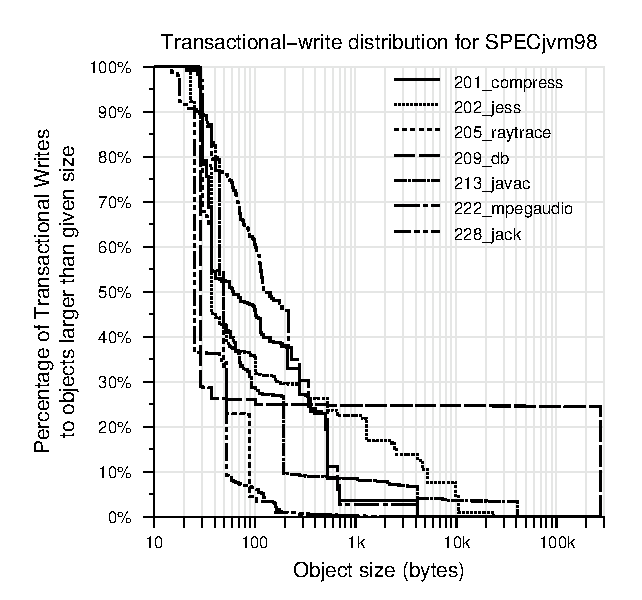
\epsfig{file=Figures/tr-w-all.eps,width=2.25in,clip=true}
\caption{Proportion of transactional writes to objects equal to or
  smaller than a given size.}
\label{fig:tr-w}%
\end{figure}%
Our software transactions implementation clones objects on
transactional writes, so that the previous state of the object can be
restored if the transaction aborts.  \figref{tr-w} shows the object
size distribution of transactional writes for SPECjvm98, and
indicates that over 10\% of writes may be to large objects.
Obviously the copying cost would be prohibitive.

Our solution is to represent large objects as \defn{functional
  arrays}.  O'Neill and Burton \cite{ONeillBu97} give a fairly
inclusive overview of such algorithms; we've chosen Tyng-Ruey Chuang's
version \cite{Chuang94} of \emph{shallow binding}, which uses
randomized cuts to the version tree to limit the cost of a read to
$O(n)$ in the worst case.  Single-threaded accesses to the array are
$O(1)$.  Our use of functional arrays is single-threaded in the common
case, when transactions do not abort.  Chuang's scheme is attractive
because it limits the worst-case cost of an abort, with very little
added complexity.

Of course, Chuang's algorithm is not lock free.
The crucial operation is a rotation of a \emph{difference node} with the
main body of the array.  Elsewhere we present a lock-free version of
Chuang's algorithm~\cite{Ananian05}; for the purposes of the present paper we
can obtain a trivial implementation using some
existing small-transaction HTM.

\subsection{Hybrid STM/HTM}\label{sec:hybrid}
\begin{figure}\centering
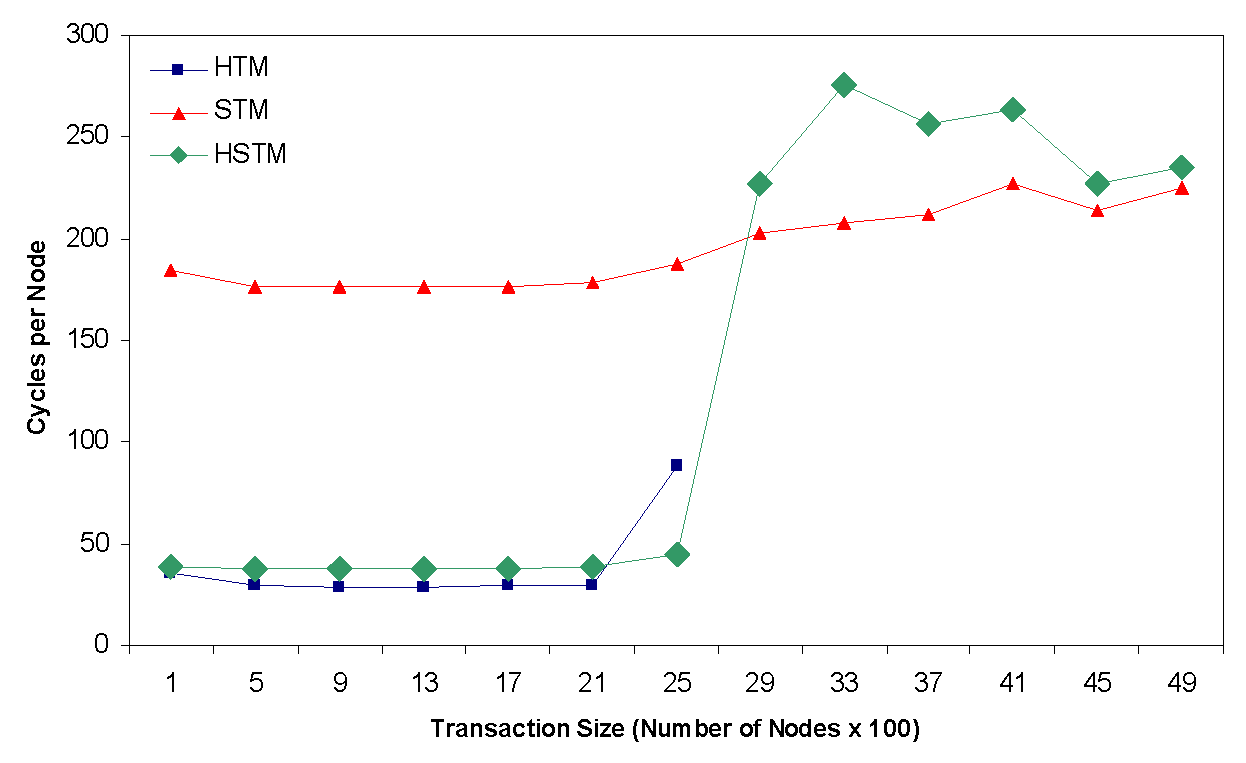
\epsfig{file=Figures/sean_lie_6b.eps,width=3.25in,clip=true}
\caption{Performance (in cycles per node push on a simple queue
  benchmark) of LTM\punt{~\cite{AnanianAsKuLeLi04}} (HTM), the
%%%%%%%%%%%%%%%%%%%^^^^^^ XXXXXXXXXXXXXXXXXXXXXXXXXXX
  object-based system presented in this paper (STM) and a hybrid
  scheme (HSTM).}%
\label{fig:hybrid}%
\end{figure}
It is worth considering if a low-level HTM can yield benefits other
than efficient implementations of large-object operations.  In fact,
\figref{hybrid} presents research showing that we can combine the
strengths of our object-based software transaction system with a
fast bounded-size HTM.  In the figure, combining the systems is done
in the most simple-minded way: all transactions are begun in
LTM~\cite{AnanianAsKuLeLi04},
and after any abort the transaction is restarted in the
object-based software system.  The field flag mechanism described in
\secref{flagfield} ensures that software transactions properly abort
conflicting hardware transactions; hardware transactions must perform
the \texttt{ReadNT} and \texttt{WriteNT} algorithms for a slight
overhead (as shown in the figure).

\secput{verification}{Verification}
The Promela model of this software transaction system was model
checked with Spin version 4.1.0 and verified to operate correctly and
without races in the scenarios described below.  The verification was
done on an SGI 64-processor MIPS machine with 16G of memory.

Sequences of transactional and non-transactional load and store
operations were checked using two concurrent processes,
\punt{
\footnote{Spin is not particularly suited to checking models with dynamic
allocation and deallocation.  In particular, the order of allocation
artificially enlarges the state space.
A great deal of effort was expended tweaking the
model to approach a canonical allocation ordering.  A better solution
to this problem would allow larger model instances to be checked.}
}
and all possible
interleavings were found to produce results consistent with
the semantic atomicity of the transactions.  A number of subtle race
conditions were discovered and corrected during this process.
In particular, early versions of the algorithms sometimes allowed
readers to escape being aborted while racing a writer in
\texttt{createVersion}, and could allow inconsistent reads.

\punt{
\secput{related}{Related work}
A number of researchers have been investigating transactional memory
systems.  This is the first paper to present a model-checked non-blocking
object-based system that allows co-existence of non-transactional and
transactional accesses to a dynamic set of object fields.

The first proposal for software transactional memory was proposed by
Shavit and Touitou \cite{ShavitTo95}; their system requires that all
input and output locations touched by a transaction be known in
advance, which limits its application.  It performs at least 10
fetches and 4 stores per location accessed (not counting the loads and
stores directly required by the computation).  The benchmarks
presented were run on between 10 and 64 processors.

Rudys and Wallach \cite{RudysWa02} proposed a copying-based
transaction system to allow rollback of hostile codelets.
They show an order of magnitude slowdown for field and array
accesses, and 6x to 23x slowdown on their benchmarks.

Herlihy, Luchangco, Moir, and Scherer's scheme \cite{HerlihyLuMoSc03}
allows transactions to touch a dynamic set of memory locations;
however the user still has to explicitly \emph{open} every object touched
before it can be used in a transaction.  This implementation is based
on object copying, and so has poor performance for large objects and
arrays.  Not including work necessary to copy objects involved in
writes, they require $O(R(R+W))$ work to open $R$ objects for reading
and $W$ objects for writing, which may be quadratic in the number of objects
involved in the transaction.   A list insertion benchmark that they
present shows 9x slowdown over a locking scheme, they beat the locking
implementation when more than 5-10 processors are active.  They
present benchmark data with up to 576 threads on 72 processors.

Harris and Fraser built a software transaction system on a flat
word-oriented transactional memory abstraction \cite{HarrisFr03},
roughly similar to simulating Herlihy's original hardware
transactional memory proposal in software.  This avoids problems with
large objects.  Performing $m$ memory operations touching $l$ distinct
locations costs at least $m+l$ extra reads and $l+1$ CAS operations, in
addition to the reads and writes required by the computation.
They appear to execute about twice as slowly as a locking
implementation on some microbenchmarks.  They benchmark on a
4-processor as well as a 106-processor machine; their crossover point
(at which the blocking overhead of locks matches the software
transaction overhead) is around 4 processors.
Note that Harris and Fraser do not address the problem of
concurrent non-transactional operations on locations involved in a
transaction.  Java synchronization allows such concurrent operations,
with semantics given by the Java memory model \cite{MansonPu02}.
We support these operations safely using our \FLAG mechanism.
}
%%%%%%%%%%%%%%%%%%%%%%%%%%%%%%%
\punt{
Ideas:
 - virtual memory/overlays comparison
 - what is expensive in software versions XBEGIN?  XLD?
 - basic ideas of software impls
   also, how they handle overflow & other limits.
 - honest about what we're showing.
   here's what happens if you explore the hardware avenue.
   sw technology problems become solved hw problems.
 - k-compare-and-swap insufficient?
 - say when we couldn't find performance numbers.
   performance #s in terms of reads/writes.
 - now that we know what transactions look like,
   we want to use BTM\@.
 - use categories?
 - STM systems always use ridiculously large # processors for benchmarks.

The software just ain't good enough!
\begin{itemize}
\item Argue that SW isn't good
\item Also, lots of transactional loads and stores
\end{itemize}

Software transactional memory implementations:
% FOR EACH: PERFORMANCE.  IDEA.  LIMITS.
\begin{itemize}
\item Shavit and Touitou \cite{ShavitTo95}: static transactions only;
  that is, input and output locations must be known in advance.
  Performance?
  Non-blocking, based on LL/SC. k-word compare\&swap operation.
  ``outperforms Herlihy's translation method for sufficiently large
  numbers of processors.''  Alleges Herlihy/Moss is blocking?
  I think this is actually the case.  Our scheme is not.
  Elsewhere, ``but not non-blocking, since a single process which is
  repeatedly swapped during the execution of a transaction will never
  terminate successfully''.  They define non-blocking as ``repeated
  execution of some transaction by a process implies that some process
  (not necessarily the same one and with a possibly different
  transaction) will terminate successfully after a finite number of
  attempts in the whole system.''
  ``static transactions, that is, transactions which access a
  pre-determined sequence of locations.  This class includes most of
  the known and proposed synchronization primitives in the
  literature.''
  Requires one ownership record for every location in the memory.
  no limits to size of trans, since we allocate one ownership record
  per memory location.

  Performance: *at least* 5 fetches, 5 LL, and 4SC per location
  accessed.

  64 processors; no numbers presented for less than 10 processors.

  acquire/release/agree are expensive.

\item Rudys and Wallach \cite{RudysWa02}: transactions for security.
  6x to 23x slowdown.  Creates 'backup' objects.  Predictably bad
  for large objects.  10x slowdown for field/array accesses.
  only uniprocessor.

\item Herlihy et al \cite{HerlihyLuMoSc03}: dynamic transactions, but
  copies entire object and so works for small objects only.  Basically
  Herlihy's method.  You must explicitly \emph{open} every object
  accessed, at which time conflict-checking is done.
  O((R+W)R) work to open R objects for reading and W objects for
  writing, plus cost to copy W objects once.  Concretely: for simple
  list insert/delete, locks perform 768 ops/ms, and best DSTM scheme
  is 80 ops/ms.   So over 9x slowdown.
  Up to 576 threads on 72 processors.

  open and commit are the expensive operations.
\item Harris and Fraser \cite{HarrisFr03}: atomic sections, word-based
  scheme.  no safety for non-transactional operations which might
  touch transactional locations.  transactional operation at least 2x
  slower than normal op.
  XBEGIN = CAS + STORE
  XFAIL = STORE
  Tread = 2 FETCH (best case)
  Twrite = 1 FETCH + (1 FETCH and 2 STOREs, on same cache line)
  XEND = > (1 FETCH + 1 CAS) for each distinct word read or written.

  overhead of a committing transaction performing r reads and w writes
  to 'l' distinct locations.
  is at least (2r+2w+(l)) reads (2w+1) writes, and (l+1) CAS
  operations.  2(r+w)+l reads, 2w+1 writes, and (l+1) CAS operations.

m memory operations to l locations does m+l extra reads and l+1 CAS operations.

  4 proc; also 48 proc of 106-processor machine.  I think the
  crossover point is around 4 proc.

  COMMIT is the most expensive operation.
\end{itemize}
}


\secput{concl}{Conclusions}
We have described an efficient object-based implementation of
non-blocking software transactions, along with empirical data backing
its design and extensions for large objects and HTM hybridization.
The design has been checked with the Spin model checker, and
implemented in the FLEX Java compiler.

\section*{Spin model for Software Transactions}
The complete Spin 4.1.0 model for the FLEX software transaction system is
available for download at
\url{http://flex-master.csail.mit.edu/Harpoon/swx.pml}.

\section*{Acknowledgments}
The work described in \secref{hybrid} was joint with Sean Lie, who provided
\figref{hybrid}.

\small
\bibliographystyle{abbrv}
\bibliography{xaction}

\clearpage
\normalsize
\appendix
\secput{promela}{Promela Primer}
A concise Promela reference is available at
\url{http://spinroot.com/spin/Man/Quick.html}; we will here attempt to
summarize just enough of the language to allow the model we've
presented in this paper to be understood.

Promela syntax is C-like, with the same lexical and commenting
conventions.  Statements are separated by either a semi-colon, or,
equivalently, an arrow.  The arrow is typically used to separate a
guard expression from the statements it is guarding.

The program counter moves past a statement only if the statement is
{\it enabled}.  Most
statements, including assignments, are always enabled.
A statement consisting only of an expression is enabled iff the
expression is true (non-zero).
Our model uses three basic Promela statements: selection, repetition,
and {\tt atomic}.

The selection statement,
\begin{inlinecode}
if
:: guard -> statements
...
:: guard -> statements
fi
\end{inlinecode}
selects one among its options and executes it.  An option can be
selected iff its first statement (the guard) is enabled.  The
special guard {\tt else} is enabled iff all other guards are not.

The repetition statement,
\begin{inlinecode}
do
:: statements
...
:: statements
fi
\end{inlinecode}
is similar: one among its enabled statements is selected and executed,
and then the process is repeated (with a different statement possibly
being selected each time) until control is explicitly transfered out
of the loop with a {\tt break} or {\tt goto}.

Finally,
\begin{inlinecode}
atomic { statements }
\end{inlinecode}
executes the given statements in one indivisible step.  For the
purposes of this model, a {\tt d\_step} block is functionally identical.
Outside {\tt atomic} or {\tt d\_step} blocks, Promela allows
interleaving before and after every statement, but statements are
indivisible.

Functions as specified in this model are similar to C macros: every
parameter is potentially both an input {\it and} an output.  Calls to
functions with names starting with {\tt move} are simple assignments;
they've been turned into macros so that reference counting
can be performed.

\punt{
\subsection{A simple implementation of functional arrays}
Our atomic method implementation will use \emph{functional arrays} as
a building block.  Functional arrays are \emph{persistent}; that is,
after an element is updated both the new and the old contents of the
array are available for use.  Since arrays are simply maps from
integers (indexes) to values; any functional map datatype (for
example, a functional balanced tree) can be used to implement
functional arrays.

However, the distinguishing characteristic of an imperative array is its
theoretical complexity: $O(1)$ access or update of any element.
Implementing functional arrays with a functional balanced tree yields
$O(\lg n)$ worst-case access or update.
% We will address this
% discrepancy in Section~\ref{sec:large-obj}.

For concreteness, functional arrays have the following three
operations defined:
\begin{itemize}
\item $\funcname{FA-Create}(n)$: Return an array of size $n$.  The contents of
  the array are initialized to zero.
\item $\funcname{FA-Update}(A_j, i, v)$: Return an array $A_{j'}$ that is
  functionally identical to array $A_j$ except that $A_{j'}(i)=v$.
  Array $A_j$ is not destroyed and can be accessed further.
\item $\funcname{FA-Read}(A_j, i)$: Return $A_j(i)$.
\end{itemize}
We allow any of these operations to \emph{fail}.  Failed operations
can be safely retried, as all operations are idempotent by definition.

For the moment, consider the following na{\"\i}ve implementation:
\begin{itemize}
\item $\funcname{FA-Create}(n)$: Return an ordinary imperative array of size
  $n$.
\item $\funcname{FA-Update}(A_j, i, v)$: Create a new imperative array
  $A_{j'}$ and copy the contents of $A_j$ to $A_{j'}$.  Return $A_{j'}$.
\item $\funcname{FA-Read}(A_j, i)$: Return $A_j[i]$.
\end{itemize}
This implementation has $O(1)$ read and $O(n)$ update, so it matches
the performance of imperative arrays only when $n=O(1)$.  We will
therefore call these \emph{small object functional arrays}.  Operations
in this implementation never fail.  Every operation is non-blocking
and no synchronization is necessary, since the imperative arrays are
never mutated after they are created.

\subsection{A single-object protocol}
\begin{figure}\centering
\includegraphics[width=3.25in,clip=true]{Figures/nb-single-obj.eps}
\figadjust%
\caption{Implementing non-blocking single-object concurrent operations
  with functional arrays.}
\label{fig:single-o}
\end{figure}
Given a non-blocking implementation of functional arrays, we can
construct an implementation of \atomic for single objects.  In
this implementation, fields of at most one object may be referenced
during the execution of the atomic method.

We will consider the following two operations on objects:
\begin{itemize}
\item $\funcname{Read}(o, f)$: Read field $f$ of $o$.  We will assume that
  there is a constant mapping function that given a field name
  returns an integer index.  We will write the result of mapping $f$
  as \fref{f}{index}.  For simplicity, and without loss of generality,
  we will assume all fields are of equal size.
\item $\funcname{Write}(o, f, v)$: Write value $v$ to field $f$ of $o$.
\end{itemize}
All other operations on Java objects, such as method dispatch and type
interrogation, can be performed using the immutable {\tt type}
field in the object.  Because the {\tt type} field is never changed
after object creation, non-blocking implementations of operations on
the {\tt type} field are trivial.

As Figure~\ref{fig:single-o} shows, our single-object implementation
of \atomic represents objects as a pair, combining {\tt type} and a
reference to a functional array.  When not inside an atomic
method, object reads and writes are implemented using the
corresponding functional array operation, with the array reference in
the object being updated appropriately:
\begin{itemize}
\item $\funcname{Read}(o, f)$:
  Return $\funcname{FA-Read}(\fref{o}{fields}, \fref{f}{index})$.
\item $\funcname{Write}(o, f, v)$: Replace \fref{o}{fields} with the
  result of $\funcname{FA-Update}(\fref{o}{fields}, \fref{f}{index}, v)$.
\end{itemize}

The interesting cases are reads and writes inside an atomic method.
At entry to our atomic method that will access (only) object $o$, we
store \fref{o}{fields} in a local variable $u$.  We create another
local variable $u'$ which we initialize to $u$.  Then our read and
write operations are implemented as:
\begin{itemize}
\item $\funcname{ReadAtomic}(o, f)$:
  Return $\funcname{FA-Read}(u', \fref{f}{index})$.
\item $\funcname{WriteAtomic}(o, f, v)$:
  Update variable $u'$ to the result of
  $\funcname{FA-Update}(u', \fref{f}{index}, v)$.
\end{itemize}

At the end of the atomic method, we use Compare-And-Swap to atomically
set \fref{o}{fields} to $u'$ iff it contained $u$.  If the CAS fails,
we back-off and retry.

With our na{\"\i}ve ``small object'' functional arrays, this implementation is
exactly the ``small object protocol'' of Herlihy \cite{Herlihy93}.
Herlihy's protocol is rightly criticized for an excessive amount of
copying.  We will address this with a better implementation of
functional arrays in Section~\ref{sec:large-obj}.
However, the restriction that only one object
may be referenced within an atomic method is overly limiting.

\subsection{Extension to multiple objects}
\begin{figure}[t]\centering
\includegraphics[width=3.25in,clip=true]{Figures/nb-multi-obj.eps}
\figadjust%
\caption{Data structures to support non-blocking multi-object
  concurrent operations.  Objects point to a linked list of versions,
  which reference operation identifiers.  Versions created within the
  same execution of an atomic method share the same operation
  identifier.  Version structure also contain pointers to functional
  arrays, which record the values for the fields of the object.
  If no modifications have been made to the object, multiple versions
  in the list may share the same functional array.}
\label{fig:multi-o}
\end{figure}
\begin{figure}[p]
\renewcommand{\>}{~~}
\newcommand{\com}[1]{\hfill [{\sl #1}]}
\begin{tabular}{l}
$\funcname{Read}(o, f)$:\\
begin\\
retry:\\
\>$u \gets \fref{o}{versions}$ \\
\>$u' \gets \fref{u}{next}$ \\
\>$s  \gets \fref{\fref{u}{owner}}{status}$ \\
\>if ($s=\text{\sl DISCARDED}$) \com{Delete DISCARDED?}\\
\>\>CAS$(u, u', \addr{\fref{o}{versions}})$\\
\>\>goto retry \\
\>else if ($s=\text{\sl COMPLETE}$)\\
\>\>$a \gets \fref{u}{fields}$ \com{$u$ is COMPLETE}\\
\>\>$\fref{u}{next} \gets \text{\bf null}$ \com{Trim version list}\\
\>else\\
\>\>$a \gets \fref{u'}{fields}$ \com{$u'$ is COMPLETE}\\
\>return $\funcname{FA-Read}(a, \fref{f}{index})$ \com{Do the read}\\
end\\
\\
$\funcname{ReadAtomic}(o, f)$:\\
begin\\
\>$u \gets \fref{o}{versions}$\\
\>if ($\var{oid} = \fref{u}{owner}$) \com{My OID should be first}\\
\>\>return $\funcname{FA-Read}(\fref{u}{fields}, \fref{f}{index})$
\com{Do the read}\\
\>else \com{Make me first!}\\
\>\>$u' \gets \fref{u}{next}$\\
\>\>$s  \gets \fref{\fref{u}{owner}}{status}$\\
\>\>if ($s=\text{\sl DISCARDED}$) \com{Delete DISCARDED?}\\
\>\>\>CAS$(u, u', \addr{\fref{o}{versions}})$\\
\>\>else if ($\fref{\var{oid}}{status}=\text{\sl DISCARDED}$)
\com{Am I alive?}\\
\>\>\>fail\\
\>\>else if ($s=\text{\sl IN-PROGRESS}$) \com{Abort IN-PROGRESS?}\\
\>\>\>CAS$(s, \text{\sl DISCARDED}, \addr{\fref{\fref{u}{owner}}{status}})$\\
\>\>else \com{Link new version in:} \\
\>\>\>$\fref{u}{next} \gets \text{\bf null}$ \com{Trim version list}\\
\>\>\>$u' \gets \text{new \tt Version}(\var{oid}, u, \text{\bf null})$
\com{Create new version}\\
\>\>\>if (CAS$(u, u', \addr{\fref{o}{versions}}) \neq \text{\sl FAIL}$)\\
\>\>\>\>$\fref{u'}{fields} \gets \fref{u}{fields}$ \com{Copy old fields}\\
\>\>goto retry\\
end\\
\end{tabular}
\figadjust%
\caption{\funcname{Read} and \funcname{ReadAtomic} implementations for the
  multi-object protocol.}\label{fig:reads}
\end{figure}

\begin{figure}[p]
\renewcommand{\>}{~~}
\newcommand{\com}[1]{\hfill [{\sl #1}]}
\begin{tabular}{l}
$\funcname{Write}(o, f, v)$:\\
begin\\
retry:\\
\>$u  \gets \fref{o}{versions}$\\
\>$u' \gets \fref{u}{next}$\\
\>$s  \gets \fref{\fref{u}{owner}}{status}$\\
\>if ($s=\text{\sl DISCARDED}$) \com{Delete DISCARDED?}\\
\>\>CAS$(u, u', \addr{\fref{o}{versions}})$\\
\>else if ($s=\text{\sl IN-PROGRESS}$) \com{Abort IN-PROGRESS?}\\
\>\>CAS$(s, \text{\sl DISCARDED}, \addr{\fref{\fref{u}{owner}}{status}})$\\
\>else \com{$u$ is COMPLETE}\\
\>\>$\fref{u}{next} \gets \text{\bf null}$ \com{Trim version list}\\
\>\>$a \gets \fref{u}{fields}$\\
\>\>$a' \gets \funcname{FA-Update}(a, \fref{f}{index}, v)$\\
\>\>if (CAS$(a, a', \addr{\fref{u}{fields}}) \neq \text{\sl FAIL}$)
\com{Do the write}\\
\>\>\>return \com{Success!}\\
\>goto retry\\
end\\
\\
$\funcname{WriteAtomic}(o, f, v)$:\\
begin\\
\>$u  \gets \fref{o}{versions}$\\
\>if ($oid = \fref{u}{owner}$) \com{My OID should be first}\\
\>\>$\fref{u}{fields} \gets \funcname{FA-Update}(\fref{u}{fields}, \fref{f}{index}, v)$\com{Do write}\\
\>else \com{Make me first!}\\
\>\>$u' \gets \fref{u}{next}$\\
\>\>$s  \gets \fref{\fref{u}{owner}}{status}$\\
\>\>if ($s=\text{\sl DISCARDED}$) \com{Delete DISCARDED?}\\
\>\>\>CAS$(u, u', \addr{\fref{o}{versions}})$\\
\>\>else if ($\fref{\var{oid}}{status}=\text{\sl DISCARDED}$)
\com{Am I alive?}\\
\>\>\>{\it fail}\\
\>\>else if ($s=\text{\sl IN-PROGRESS}$) \com{Abort IN-PROGRESS?}\\
\>\>\>CAS$(s, \text{\sl DISCARDED}, \addr{\fref{\fref{u}{owner}}{status}})$\\
\>\>else \com{Link new version in:} \\
\>\>\>$\fref{u}{next} \gets \text{\bf null}$ \com{Trim version list}\\
\>\>\>$u' \gets \text{new \tt Version}(\var{oid}, u, \text{\bf null})$
\com{Create new version}\\
\>\>\>if (CAS$(u, u', \addr{\fref{o}{versions}}) \neq \text{\sl FAIL}$)\\
\>\>\>\>$\fref{u'}{fields} \gets \fref{u}{fields}$ \com{Copy old fields}\\
\>\>goto retry\\
end\\
\end{tabular}
\figadjust%
\caption{\funcname{Write} and \funcname{WriteAtomic} implementations for the
  multi-object protocol.}\label{fig:writes}
\end{figure}

We now extend the implementation to allow the fields of any number of
objects to be accessed during the atomic method.
Figure~\ref{fig:multi-o} shows our new object representation.
Objects consist of two slots, and the first represents the immutable
{\tt type}, as before.  The second field, {\tt versions}, points to a
linked list of {\tt Version} structures.  The {\tt Version} structures
contain a pointer {\tt fields} to a functional array, and a pointer
{\tt owner} to an \emph{operation identifier}.  The operation
identifier contains a single field, {\tt status}, which can be set to
one of three values: \textsl{COMPLETE}, \textsl{IN-PROGRESS}, or
\textsl{DISCARDED}.  When the operation identifier is created, the
status field is initialized to \textsl{IN-PROGRESS}, and it will be
updated exactly once thereafter, to either \textsl{COMPLETE} or
\textsl{DISCARDED}.  A \textsl{COMPLETE} operation identifier never
later becomes \textsl{IN-PROGRESS} or \textsl{DISCARDED}, and
a \textsl{DISCARDED} operation identifier never becomes
\textsl{COMPLETE} or \textsl{IN-PROGRESS}.

We create an operation identifier when we begin or restart an atomic
method and place it in a local variable \emph{oid}.  At the end of the
atomic method, we use CAS to set \fref{\var{oid}}{status} to
{\sl COMPLETE} iff it was {\sl IN-PROGRESS}.  If the CAS is successful,
the atomic method has also executed successfully; otherwise
$\fref{\var{oid}}{status}=\text{\sl DISCARDED}$ and we must
back-off and retry the atomic method.  All {\tt Version} structures
created while in the atomic method will reference \emph{oid} in
in their {\tt owner} field.

Semantically, the current field values for the object will be given by
the first version in 
the versions list whose operation identifier is {\sl COMPLETE}.
This allows us to link {\sl IN-PROGRESS} versions in at the head of
multiple objects' versions lists and atomically change the values of
all these objects by setting the one common operation identifier to
{\sl COMPLETE}.  We only allow one {\sl IN-PROGRESS} version on the
versions list, and it must be at the head, so
Therefore, before we can link a new version at the head, we
must ensure that every other version on the list is {\sl DISCARDED} or
{\sl COMPLETE}.

Since we will never look past the first {\sl COMPLETE} version in the
versions list, we can free all versions past that point.  In our
presentation of the algorithm, we do this by explicitly setting the
{\tt next} field of every {\sl COMPLETE} version we see to {\bf null};
this allows the versions past that point to be garbage collected.
An optimization would be to have the garbage collector do the list
trimming for us when it does a collection.
% always must read u.next before u.owner.status to ensure we don't
% get caught with a null pointer from a version that just committed.

We don't want to inadvertently chase the null {\tt next} pointer
of a {\sl COMPLETE} version, so we always load the {\tt next}
field of a version \emph{before} we load {\tt owner.status}.  Since
the writes occur in the reverse order ({\sl COMPLETE} to
{\tt owner.status}, then {\bf null} to {\tt next}) we have ensured that
our {\tt next} pointer is valid whenever the status is not {\sl COMPLETE}.

We begin an atomic method with \funcname{AtomicEntry} and attempt to
complete an atomic method with \funcname{AtomicExit}.  They are defined as
follows:
\begin{itemize}
\item $\funcname{AtomicEntry}$: create a new operation identifier, with
  its status initialized to {\sl IN-PROGRESS}.  Assign it to the
  thread-local variable \var{oid}.
\item $\funcname{AtomicExit}$:
  If
 $$\text{CAS}(\text{\sl IN-PROGRESS}, \text{\sl COMPLETE},
             \addr{\fref{\var{oid}}{status}})$$
  is successful, the atomic method as a whole has completed successfully,
  and can be linearized at the location of the CAS.
  Otherwise, the method has failed.  Back-off and retry from
  \funcname{AtomicEntry}.
\end{itemize}
Pseudo-code describing \funcname{Read}, \funcname{Write}, \funcname{AtomicRead},
and \funcname{AtomicWrite} is presented in Figures~\ref{fig:reads} and
\ref{fig:writes}.  In the absence of contention, all operations take
constant time plus an invocation of \funcname{FA-Read} or
\funcname{FA-Update}.

\subsection{Lock-free functional arrays}\label{sec:large-obj}
\begin{figure*}\centering
\includegraphics[width=7in,clip=true]{Figures/chuang.eps}
\figadjust%
\caption{Shallow binding scheme for functional arrays, from
  \cite[Figure~1]{Chuang94}.}
\label{fig:chuang}
\end{figure*}
In this section we will present a lock-free implementation of functional
arrays with $O(1)$ performance in the absence of contention.  This
will complete our implementation of non-blocking \atomic methods for Java.

There have been a number of proposed implementations of functional
arrays, starting from the ``classical'' functional binary tree
implementation.  O'Neill and Burton \cite{ONeillBu97} give a fairly
inclusive overview.  Functional array implementations fall generally
into one of three categories: \emph{tree-based}, \emph{fat-elements},
or \emph{shallow-binding}.

Tree-based implementations typically have a logarithmic term in their
complexity.  The simplest is the persistent binary tree with $O(\ln
n)$ look-up time; Chris Okasaki 
\cite{Okasaki95} has implemented a purely-functional random-access list
with $O(\ln i)$ expected lookup time, where $i$ is the index of the
desired element.

Fat-elements implementations have per-element data structures indexed
by a master array. Cohen \cite{Cohen84} hangs a list of
versions from each element in the master array.
O'Neill and Burton \cite{ONeillBu97}, in a more sophisticated
technique, hang a splay tree off each element and achieve $O(1)$
operations for single-threaded use, $O(1)$ amortized cost when
accesses to the array are ``uniform'', and $O(\ln n)$ amortized worst
case time. 

Shallow binding was introduced by Baker \cite{Baker78} as a method to
achieve fast variable lookup in Lisp environments.  Baker clarified
the relationship to functional arrays in \cite{Baker91}.  Shallow
binding is also called \emph{version tree arrays}, \emph{trailer
  arrays}, or \emph{reversible differential lists}.  A typical
drawback of shallow binding is that reads may take $O(u)$ worst-case
time, where $u$ is the number of updates made to the array.  Tyng-Ruey
Chuang \cite{Chuang94} uses randomized cuts to the version tree to limit
the cost of a read to $O(n)$ in the worst case.  Single-threaded
accesses are $O(1)$.

Our use of functional arrays is single-threaded in the common case,
when transactions do not abort.  Chuang's scheme is attractive because
it limits the worst-case cost of an abort, with very little added
complexity.   In this section we will present a lock-free version of
Chuang's randomized algorithm.

In shallow binding, only one version of the functional array (the
\emph{root}) keeps its contents in an imperative array (the
\emph{cache}).   Each of the other versions is represented as a path
of \emph{differential nodes}, where each node describes the
differences between the current array and the previous array.  The
difference is represented as a pair \tuple{\text{\it index},\text{\it value}},
representing the new value to be stored at the specified index.
All paths lead to the root.  An update to the functional array is
simply implemented by adding a differential node pointing to the array it is
updating.

The key to constant-time access for single-threaded use is provided by the read
operation.  A read to the root simply reads the appropriate value from
the cache.  However, a read to a differential node triggers a series
of rotations that swap the direction of differential nodes and result
in the current array acquiring the cache and becoming the new root.
This sequence of rotations is called \emph{re-rooting}, and is
illustrated in Figure~\ref{fig:chuang}.  Each rotation
exchanges the root nodes for a differential node pointing to it, after
which the differential node becomes the new root and the root becomes
a differential node pointing to the new root. The cost of a read is
proportional to its re-rooting length, but after the first read
accesses to the same version are $O(1)$ until the array is re-rooted again.

Shallow binding performs badly if read operations ping-pong between two
widely separated versions of the array, as we will continually
re-root the array from one version to the other.
Chuang's contribution is to provide for \emph{cuts} to the chain of
differential nodes: once in a while we clone the cache and create a
new root instead of performing a rotation.  This operation takes
$O(n)$ time, so we amortize it over $n$ operations by randomly
choosing to perform a cut with probability $1/n$.

\begin{figure*}\centering
\includegraphics[width=7in,clip=true]{Figures/funarr.eps}
\figadjust%
\caption{Atomic steps in $\funcname{FA-Rotate}(B)$.  Time proceeds top-to-bottom
  on the left hand side, and then top-to-bottom on the right.
  Array $A$ is a root node, and $\funcname{FA-Read}(A, x)=z$.
  Array $B$ has the almost the same contents as $A$, but
  $\funcname{FA-Read}(B, x)=y$.}
\label{fig:funarr}
\end{figure*}

\begin{figure*}\centering
\renewcommand{\>}{~~}
\newcommand{\com}[1]{\hfill [{\sl #1}]}
\begin{tabular}{l}
$\funcname{FA-Update}(A, i, v)$:\\
begin\\
\>$d \gets \text{new DiffNode}(i, v, A)$\\
\>$A'\gets \text{new Array}(\fref{A}{size}, d)$\\
\>return $A'$\\
end\\
\\
$\funcname{FA-Read}(A, i)$:\\
begin\\
retry:\\
\>$d_C \gets \fref{A}{node}$\\
\>if $d_C$ is a cache, then\\
\>\>$v \gets \fref{A}{node}[i]$\\
\>\>if $(\fref{A}{node} \neq d_C)$\com{consistency check}\\
\>\>\>goto retry\\
\>\>return $v$\\
\>else\\
\>\>\funcname{FA-Rotate}(A)\\
\>\>goto retry\\
end\\
\\
$\funcname{FA-Rotate}(B)$:\\
begin\\
retry:\\
\>$d_B \gets \fref{B}{node}$\com{step (1): assign names as per Figure~\ref{fig:funarr}.}\\
\>$A \gets \fref{d_B}{array}$\\
\>$x \gets \fref{d_B}{index}$\\
\>$y \gets \fref{d_B}{value}$\\
\>$z \gets \funcname{FA-Read}(A, x)$\com{rotates A as side effect}\\
\\
\>$d_C \gets \fref{A}{node}$\\
\>if $d_C$ is not a cache, then \\
\>\>goto retry\\
\\
\>if $(0 = (\text{random} \bmod \fref{A}{size}))$\com{random cut}\\
\>\>$d_C' \gets \text{copy of }d_C$\\
\>\>$d_C'[x] \gets y$\\
\>\>$s\gets\text{DCAS}(d_C, d_C, \addr{\fref{A}{node}}, d_B, d_C', \addr{\fref{B}{node}})$\\
\>\>if $(s \neq \text{\sl SUCCESS})$ goto retry\\
\>\>else return\\
\\
\>$C \gets \text{new Array}(\fref{A}{size}, d_C)$\\
\>$d_A \gets \text{new DiffNode}(x, z, C)$\\
\\
\>$s \gets \text{CAS}(d_C, d_A, \addr{\fref{A}{node}})$\com{step (2)}\\
\>if $(s\neq \text{\sl SUCCESS})$ goto retry\\
\\
\>$s\gets\text{CAS}(A, C, \addr{\fref{d_B}{array}})$\com{step (3)}\\
\>if $(s\neq \text{\sl SUCCESS})$ goto retry\\
\\
\>$s \gets\text{CAS}(C, B, \addr{\fref{d_A}{array}})$\com{step (4)}\\
\>if $(s\neq \text{\sl SUCCESS})$ goto retry\\
\\
\>$s \gets \text{DCAS}(z, y, \addr{d_C[x]},  d_C, d_C, \addr{\fref{C}{node}})$\com{step (5)}\\
\>if $(s\neq \text{\sl SUCCESS})$ goto retry\\
\\
\>$s \gets \text{DCAS}(d_B, d_C, \addr{\fref{B}{node}}, d_C, {\bf nil}, \addr{\fref{C}{node}})$\com{step (6)}\\
\>if $(s\neq \text{\sl SUCCESS})$ goto retry\\
end\\
\end{tabular}
\figadjust%
\caption{Implementation of lock-free functional array using shallow
  binding and randomized cuts.}
\label{fig:fun-impl}
\end{figure*}

Figure~\ref{fig:funarr} shows the data structures used for the
functional array implementation, and the series of atomic steps used
to implement a rotation.  The {\tt Array} class represents a
functional array; it consists of a {\tt size} for the array and a
pointer to a {\tt Node}.  There are two types of nodes: a {\tt
  CacheNode} stores a value for every index in the array, and a {\tt
  DiffNode} stores a single change to an array.  {\tt Array} objects
that point to {\tt CacheNode}s are roots.

In step 1 of the figure, we have a root array $A$ and an
array $B$ whose differential node $d_B$ points to $A$.  The functional
arrays $A$ and $B$ differ in one element: element $x$ of $A$ is $z$,
while element $x$ of $B$ is $y$.  We are about to rotate $B$ to give
it the cache, while linking a differential node to $A$.

Step 2 shows our first atomic action.  We have created a new {\tt
  DiffNode} $d_A$ and a new {\tt Array} $C$ and linked them between
$A$ and its cache.  The {\tt DiffNode} $d_A$ contains the value for
element $x$ contained in the cache, $z$, so there is no change in
the value of $A$.

We continue swinging pointers until step 5, when can finally set
the element $x$ in the cache to $y$.  We perform this operation with a
DCAS operation that checks that $\fref{C}{node}$ is still pointing to
the cache as we expect.  Note that a concurrent rotation would swing
$\fref{C}{node}$ in its step 1.  In general, therefore, the location
pointing to the cache serves as a reservation on the cache.

Thus in step 6 we need to again use DCAS to simultaneously swing
$\fref{C}{node}$ away 
from the cache as we swing $\fref{B}{node}$ to point to the cache.

Figure~\ref{fig:fun-impl} presents pseudocode for \funcname{FA-Rotate},
\funcname{FA-Read}, and \funcname{FA-Update}.  Note that \funcname{FA-Read} also
uses the cache pointer as a reservation,
double-checking the cache pointer after it finishes its read to ensure that the
cache hasn't been stolen from it.

Let us now consider cuts, where \funcname{FA-Read} clones the cache
instead of performing a rotation.   Cuts also check the cache pointer
to protect against concurrent rotations.  But what if the cut occurs
while a rotation is mutating the cache in step 5?  In this case the
only array adjacent to the root is $B$, so the cut must be occurring
during an invocation of $\funcname{FA-Rotate}(B)$.  But then the
differential node $d_B$ will be applied after the cache is copied,
which will safely overwrite the mutation we were concerned about.

Note that with hardware support for small transactions \cite{HerlihyMo93}
we could cheaply perform the entire rotation atomically, instead of
using this six-step approach.


%% \subsection{Optimizations}
%% Re-rooting is the most complicated part of the functional array
%% algorithm.  It can be optimized in a number of ways.  For example,

%% %unsync rotate for transaction-local data.
%% The first is to recognize that some array versions can only be seen by
%% a single thread.  In particular, when we are working on an {\sl
%%   IN-PROGRESS} operation, all array versions that it creates are
%% unreachable from other threads until the operation is committed.
%% We can add a field {\tt creator} to the {\tt Array} object that records what
%% operation created that version.  If the {\tt creator} field of both
%% $A$ and $B$ contains our own \var{oid} when we begin a rotate, we know
%% that these versions are both thread local

%% .. uh, no.  This doesn't work.

%% % scales method of tagging fields.


\subsecput{os}{Operating systems}

Perhaps the most promising single application for boundless
transactions is providing atomicity within an operating system.
Locking is difficult to reason about For example, we counted at the
comments in the Linux filesystem layer, and found that about 15\% of
the comments relate to locking protocols.  Those comments often
describe global invariants of the program that are difficult to
verify.  And many kernel bugs involve races and deadlocks.

[Dealing with nested transactions: modularity, semantics.]

\subsecput{htm}{HTM versus STM}

\subsecput{performance}{Performance improvements}

\note{This text may very well belong in some other section.}  Herlihy
and Moss' HTM scheme is not non-blocking.  In their proposal, a
transactional load by a processor ends with an XABORT and an XCOMMIT
tag on the read cache line.  Later, while that processor's transaction
is still outstanding, a transactional store by a different processor
to that same cache line will result in a T\_RFO cycle on the bus, to
which the first processor's cache will result BUSY.  The second
processor commits suicide (aborts itself) in response.

[A processor that does transactional reads holds an irrevocable lock
on those cache lines until it commits or aborts itself, and any
other processor that attempts a write on those lines will block,
waiting.]

This means that a processor that transactionally reads many locations
and then loops forever without committing may prevent all other
processors from ever making progress on their transactions.  This is a
simple protocol error: the intervening processor should be able to
abort the first processor instead of blocking for its completion.
Loosely, processors must be able to kill others; if a processor can
only commit suicide, than the system may block.  When transactions are
exposed to user code, Herlihy's system is vulnerable to this simple
denial-of-service attack.  BTM does not suffer from this
problem. [although starvation may still occur.]

}% end \punt

\end{document}

% LocalWords:  csail mit edu AFRL LaMarca Alemany Felten Luchangco Shavit JVM
% LocalWords:  Touitou Okasaki Qadeer Promela backoff transactified SPECjvm HTM
% LocalWords:  transactional Herlihy Ananian Rinard atomicity STM PowerPC URL
% LocalWords:  transactification Chuang Moir
